\documentclass[12pt,a4paper]{article}
\usepackage[top=3cm,bottom=2.5cm,left=2cm,right=2cm]{geometry}
\usepackage{mathtools}
\usepackage{float}
\linespread{1.5}
\usepackage[table]{xcolor}
\usepackage{graphicx}
%{\rowcolors{3}{green!80!yellow!50}{green!70!yellow!40}
\usepackage{threeparttable}
%\usepackage{multirow}
%\setlatintextfont{Times New Roman}
\usepackage{xepersian}
%\settextfont{XB Zar}
\settextfont{XB Zar}\fontsize{12}{6}\selectfont
\setlatintextfont{Times New Roman}\fontsize{11}{6}
%\usepackage{perpage}
%\MakePerPage{footnote}



\begin{document}

\begin{center}
	{\Large \textbf{مدل‌سازی مشترک موضوع و احساس در داده‌های متنی با استفاده از شبکه‌های عصبی}}\\
\end{center}

	
\section*{چکیده}
\begin{small}
	\baselineskip=0.7cm
	امروزه در حوزه‌ی هوش مصنوعی ما به دنبال الگوریتم‌ها و ساختارهایی هستیم که با دقت بالا یک  رفتار انسانی‌ و یا فرا انسانی‌ را با بیشترین سرعت ممکن انجام دهند. با گسترش اینترنت و وب، انواع مختلف رسانه‌های اجتماعی نظیر وبلاگ‌ها و شبکه‌های اجتماعی در به یک منبع بسیار عظیم از انواع مختلف داده به ویژه داده‌‌های  متنی تبدیل شده‌اند. با پردازش این داده‌ها می‌‌توان اطلاعات سودمند و مفیدی در مورد مباحث مختلف، نظر افراد و احساس کلی‌ جامعه بدست آورد. از این جهت داشتن مدل‌هایی که کاملا خودکار به تشخیص اطلاعات مفهومی‌ و احساس در اسناد متنی بپردازند بسیار مفید است. روش‌های مدل‌سازی موضوع و استخراج اطلاعات مفهمومی از داده‌های متنی و همچنین تشخیص احساس، همواره از مهمترین مباحث مطرح شده در زمینه‌ی پردازش زبان طبیعی، و کاوش داده‌های متنی است. بیشتر مدل‌هایی که در این زمینه وجود دارند بر پایه‌ی روش‌های آماری و شبکه‌های بیزی هستند به طوری که در زمینه‌ی مدل‌سازی موضوع-احساس با استفاده از شبکه‌های عصبی تا به امروز هیچ رویکردی وجود ندارد. همچنین بیشتر رویکردهای موجود دارای محدویت‌هایی مانند پیچیدگی محاسباتی بالا هستند. در این مقاله یک ساختار جدید برای مدل‌سازی مشترک احساس-موضوع در داده‌های متنی بر پایه‌ی شبکه‌‌ی عصبی ماشین بلتزمن محدود پیشنهاد می‌‌گردد. مدل پیشنهاد شده پس از پیاده‌سازی با مدل‌های موجود مقایسه گردید. مشاهده می‌شود رویکرد پیشنهادی در بحث ارزیابی به عنوان بک مدل مولد، طبقه‌بندی احساس و بازیابی اطلاعات عملکرد بهتری نسبت به مدل‌های موجود دارد.\\
	\noindent\textbf{کلمات کلیدی: مدل‌سازی موضوع، آنالیز احساس، شبکه‌ها‌ی عصبی، ماشین بلتزمن محدود، مدل احتمالاتی، الگوریتم واگرایی مقابله}
\end{small} 


\section{مقدمه}


\label{sec1}

امروزه در تمام مباحث مربوط به هوش مصنوعی ما به دنبال روش‌ها، الگوریتم‌ها و ساختارهایی هستیم که بتوانند هرچه بهتر، 
به صورت خودکار و با دقت بالا یک  رفتار انسانی‌ و یا فرا انسانی‌ را با بیشترین سرعت ممکن انجام دهند. اعمالی مانند دسته‌بندی، استخراج اطلاعات مفهومی، آنالیز و برچسب گذاری داده‌ها و از جمله فعالیت‌هایی‌ می‌‌باشند که امروزه ما انجام بسیاری از آن‌ها را به ماشین‌ها واگذار می‌‌کنیم. 

در بین انواع مختلف داده، داده‌های متنی دارای سهم عظیمی‌ از نظر حجم و مقدار هستند. به خصوص با گسترش اینترنت  و وب در دهه‌ی اخیر با سرعتی‌ بسیار زیاد، انواع مختلف رسانه‌های اجتماعی نظیر وبلاگ‌ها، شبکه‌های اجتماعی و گروه‌های بحث در اینترنت به یک منبع بسیار عظیم و قوی از انواع مختلف داده و اطلاعات به  ویژه داده‌‌های  متنی تبدیل شده اند. با پردازش این داده‌ها می‌‌توان اطلاعات سودمند و مفیدی در مورد مباحث مختلف، نقطه نظر افراد و احساس کلی‌ جامعه بدست آورد.
%\cite{lin2012weakly}.
 فعالیت‌های انجام گرفته در زمینه کاوش داده‌ها به خصوص کاوش داده‌های متنی و همچنین پردازش زبان طبیعی بیشتر از هر زمینه‌ی دیگری به تلاش برای درک و فهم این حجم عظیم از داده‌های متنی مربوط می‌‌شوند. حجم عظیمی از داده‌های متنی که بدون هیچ ساختار و قاعده و قانونی‌ هستند و روز به روز مقدار آن‌ها با سرعت بسیاری چشمگیری در حال افزایش است. در این میان وجود الگوریتم‌ها و روش‌هایی که بتوانند به صورت خودکار با این حجم زیاد از داده‌های بدون ساختار ارتباط برقرار کرده و اطلاعات مفید و سودمند را از آن برای ما استخراج کنند بیش از پیش احساس می‌‌گردد.

تمرکز ما در ابن مقاله و روش پیشنهادی پردازش بر روی داده‌های متنی است. در تقابل با داده‌های متنی، هدف ما پیدا کردن توزیع موضوع‌های مختلف موجود در مجموعه‌ی اسناد پایگاه داده و همچنین توزیع کلمات و احساس همراه با هر موضوع با استفاده شبکه‌ی عصبی است. فرآیند مورد نظر در داده‌های متنی تحت عنوان مدل‌سازی موضوع شناخته می‌‌شود که در مباحث مربوط به هوش مصنوعی در دسته‌ی کارهای مربوط به یادگیری ماشین، پردازش زبان طبیعی، شبکه‌های عصبی مصنوعی و کاوش احساسات قرارمی‌‌گیرد. در بحث مدل‌سازی موضوع با استفاده از شبکه‌های عصبی در سال‌های اخیر تعداد اندکی‌ روش ارائه شده است. اما در زمینه‌‌ی مدل‌سازی مشترک احساس و موضوع با استفاده از شبکه‌های عصبی تا کنون مدلی‌ مطرح نشده و مورد آزمایش قرار نگرفته است. نتایج بهتر مدل‌های شبکه عصبی در بحث مدل‌سازی موضوع در مقایسه با روش‌های پیشین که از ساختارهای گرافی‌ و مدل‌های بیزی استفاده می‌‌کردند، همچنین عدم وجود روشی‌ برای تشخیص همزمان احساس و موضوع در داده‌های متنی با استفاده از شبکه‌های عصبی منجر به رویکرد پیشنهادی در این مقاله برای مدل‌سازی مشترک احساس و موضوع در داده‌های متنی بر پایه‌ی شبکه‌های عصبی گردید.

مدل‌سازی موضوع و استخراج اطلاعات مفهمومی از داده‌های متنی و همچنین تشخیص احساس از مهمترین مباحث مطرح شده در زمینه‌ی پردازش زبان طبیعی، و کاوش داده‌های متنی هستند. رویکردهای موجود در این زمینه با اجرا بر روی یک پایگاه داده‌ از اسناد متنی به تشخیص و مدل‌سازی موضوع‌ها، احساسات و مفاهیم همراه با هر سند متنی می‌پردازند. تشخیص احساس برای هر سند و هر موضوع در بحث بازیابی اطلاعات نیز می‌‌تواند به اندازه تشخیص اطلاعات موجود در هر متن حائز اهمیت باشد. از این جهت داشتن مدل‌هایی که به صورت اتوماتیک و کاملا خودکار به مدل‌سازی موضوع و تشخیص اطلاعات مفهومی‌ و احساس در اسناد بپردازند می‌تواند بسیار مفید باشد. بیشتر کارهایی که در این زمینه وجود دارند بر پایه‌ی رویکردهای آماری و شبکه‌های بیزی هستند که از محدودیت‌هایی مانند پیچیدگی محاسباتی بالا رنج می‌برند. در بحث شبکه‌های عصبی بر خلاف مدل‌های آماری، روشی برای مدل کردن موضوع و احساس به صورت همزمان و مشترک وجود ندارد. در این مقاله نیز در همین راستا یک رویکرد نوین‌ بر پایه‌ی شبکه‌های عصبی مصنوعی برای مدل‌سازی همزمان موضوع‌ و احساس‌ در یک مجموعه از داده‌های متنی پیشنهاد می‌گردد. رویکرد پیشنهاد شده در این مقاله یک مدل نظارت شده‌ی مولد احتمالی‌ بر پایه‌ی شبکه‌ی عصبی ماشین بلتزمن محدود است. برای آموزش در این مدل مانند سایر روش‌هایی که بر پایه‌ی ماشین بلتزمن محدود هستند از الگوریتم یادگیری واگرایی مقابله استفاده می‌‌شود.

ساختار بخش‌های بعدی در مقاله به این صورت است: ابتدا در بخش دوم به مرور کارهای پیشین در زمینه‌ی تخمین توزیع‌های احتمالی‌ در داده‌های ورودی، مدل‌سازی موضوع، تشخیص احساس و مدل‌سازی احساس‌-موضوع در داده‌های متنی می‌‌پردازیم. در بخش سوم کلیات نظری و تئوری مدل پیشنهادی بیان می‌‌شوند. در این فصل با معرفی‌ یک مدل معروف به عنوان پایه مدل جدید تعریف و قسمت‌های مختلف آن شرح داده می‌‌شوند و روابط مورد نیاز برای هر قسمت تعریف می‌‌شوند. در بخش چهارم این مقاله مراحل شبیه‌سازی مدل پیشنهادی و نتایج حاصل از آزمایش‌های بدست آمده ومفایسه با دیگر مدل‌هاارائه می‌گردد. در بخش پایانی، نتیجه‌گیری حاصل از این مقاله شرح داده خواهد شد. همچنین راهکارهایی برای بهبود و توسعه مدل پیشنهادی ارائه خواهد شد.

\section{ بررسی مدل‌های پیشین}
\label{sec2}
در این بخش روش‌های موجود را از چندین زاویه مورد نقد و بررسی‌ قرار می‌‌دهیم و بسته به ساختار، نحوه‌ی عملکرد، نوع داده‌ی ورودی و سیر تکاملی، آن‌ها را در چندین کلاس طبقه‌بندی می‌‌کنیم.

به طور کلی روش‌های مدل‌سازی موضوع به مدل‌هایی گفته می‌‌شود که یک چکیده از موضوعات موجود در یک سند یا مجمومه‌ای از اسناد را تشخیص داده و استخرج می‌‌کنند. در بررسی‌ رویکرد‌های موجود از دید ساختاری، می‌‌توان آن‌ها را در دو گروه کلی‌ طبقه‌بندی کرد. دسته‌ی اول مدل‌های گرافی‌ و بیزی و دسته‌ی دوم مدل‌های بر پایه‌ی شبکه‌های عصبی. از نظر نحوه‌ی عملکرد مدل‌های پیشین را در سه‌  کلاس مختلف قرار دارند. دسته‌ي اول روش‌هایی که تنها به مدل‌سازی موضوع می‌‌پردازند. دسته‌ی دوم روش‌هایی که به تشخیص احساس در داده‌های ورودی می‌‌پردازند. و در دسته‌‌ي سوم از نظر نحوه‌ی عملکرد روش‌هایی قرار دارند که به صورت همزمان به مدل‌سازی موضوع و احساس بر روی داده‌ی ورودی می‌‌پردازند. اگرچه باید توجه داشت که مدل‌های موجود در زمینه تشخیص احساس در دسته‌ی مدل‌های موضوعی قرار نمی‌‌گیرند و بیشتر شامل مدل‌هایی هستند که یک طبقه‌بندی دو حالته (مثبت و منفی‌) یا سه‌ حالته (منفی‌، مثبت و بی‌ طرف) را انجام می‌‌دهند. 

روش‌های پیشین از نظر نوع داده‌ی ورودی در دو کلاس متفاوت قرار می‌‌گیرند. یک گروه روش‌هایی که تنها یک نوع داده را به عنوان ورودی قبول می‌‌کنند. منظور از یک مدل داده این است که روش‌های موجود توانایی عمل کردن به صورت همزمان بر روی چند مد مختلف از داده‌ها را ندارند، و داده‌های ورودی تنها باید یک حالت داشته باشند، مثلا تنها متن و یا تنها تصویر باشند و نمی‌‌توانند ترکیبی‌ از این‌ها باشند. دسته‌ی دوم که آن‌ها را مدل‌های چندحالته می‌‌شناسیم مدل‌هایی هستند که با داده‌های چندوجهی کار می‌‌کنند. منظور از داده‌های چندوجهی آن‌هایی هستند که شامل ترکیب چند حالت مختلف از داد‌ه‌ها می‌شوند، برای مثال ترکیب متن و تصویر و یا ترکیب تصویر و صدا. 

از نقطه‌نظر سیر تکاملی می‌‌توان روش‌های موجود را در سه‌ سطح: یک مدل‌های تخمین‌زننده‌ی توزیع، دو روش‌های مدل‌سازی موضوع و سه رویکردهای تشخیص همزمان موضوع و احساس قرار داد. البته لازم به ذکر است که روش‌های تخمین توزیع که در اینجا مطرح می‌‌گردند و در بحث پردازش زبان طبیعی مورد استفاده قرار می‌‌گیرند به تنهایی در دسته‌ی مدل‌های موضوعی قرار نمی‌‌گیرند اما پایه و اساس بسیاری از مدل‌های موضوعی هستند.

در بحث مدل‌سازی موضوع، مدل‌های گرافی‌ نسبت به روش‌های شبکه‌های عصبی از قدمت بیشتری برخوردار هستند. روش پایه‌‌ای که امروزه همچنان در مرورگر‌های اینترنتی مورد استفاده قرار می‌‌گیرد، تکرار ترم-معکوس تکرار سند (tf-idf) نام دارد. این رویکرد در سال 1986 توسط Salton معرفی شد و در آن هر سند متنی به یک بردار اعدد حقیقی‌ تبدیل می‌شود که شامل نسبت‌های تعداد تکرار کلمات مختلف است و از آن برای بازیابی اطلاعات استفاده می‌شود. برای غلبه بر محدودیت‌های tf-idf محققین حوزه‌ی IR چندین مدل کاهش بعد دیگر معرفی‌ کردند که مهمترین آن‌ها مدل فهرست کردن معنایی نهفته (LSI) است که توسط Deerwester و همکاران در سال 1990 ارائه گردید. مدل LSI با استفاده از تجزیه مقدار منفرد بر روی ماتریس خروجی از مدل tf-idf یک زیرفضای خطی در فضای ویژگی‌‌های مدل tf-idf شناسایی می‌‌کند.  این روش منجر به کاهش  قابل توجهی‌ در مجموعه‌های بزرگ می‌‌گرد. همچنین Deerwester و همکاران ادعا کردند که ویژگی‌‌های بدست آماده توسط مدل LSI
که در حقیقت یک ترکیب خطی‌ از ویژگی‌‌های مدل tf-idf هستند، توانایی تشخیص بعضی‌ از ویژگی‌‌های زبانی مانند مترادف و متضاد را دارند.

برای اثبات ادعا‌های مطرح شده در مدل LSI و همچنین بررسی‌ نقاط ضعف و قدرت این مدل، روش فهرست‌سازی معنایی نهفته‌ی احتمالاتی (pLSI) 
توسط Hofmann در سال 1999 معرفی شد. مدل pLSI یک مدل مولد احتمالاتی می‌باشد که از آن به عنوان یک مدل موضوعی نیز یاد می‌شود. در روش pLSI هر کلمه از یک موضوع خاص تولید می‌‌شود و کلمه‌های مختلف در داخل یک سند ممکن است از موضوع‌های مختلفی‌ تولید شوند. مهم‌ترین مدلی‌ که در دسته‌‌ی  رویکردهایی گرافی وجود دارد مدل معروف تخصیص دیریکله‌ی پنهان (LDA) است که در سال ۲۰۰۳ توسط Blei و همکاران 
ارائه گردید و پس آن به عنوان پایه‌ی مدل‌سازی موضوعی در بخش مدل‌های گرافی قرار گرفت. در روش  LDA مانند دیگر روش‌های مدل‌سازی موضوع، هر سند متنی به صورت یک توزیع مخلوط بر روی موضوع‌های مختلف‌ که در آن هر موضوع به وسیله‌ی یک توزیع بر روی کلمه‌ها مشخص می‌‌شود در نظر گرفته می‌شود.

مدل ماشین بلتزمن محدود که به اختصار آن را RBM می‌نامیم یک شبکه عصبی دولابه‌ی (یک لایه‌ی قابل مشاهده ویک لایه‌ی پنهان) بدون‌نظارت برای تخمین توزیع داده‌های ورودی باینری است. RBM یک مدل‌ احتمالاتی مولد است که اولین بار در سال ۱۹۸۶ توسط	Smolensky و پس از آن در سال ۲۰۰۲ به شکل دیگری توسط Hinton معرفی‌ گردید. مدل شبکه‌‌ی عصبی خودکاهشی تخمین‌زننده‌ی توزیع (NADE) که از مدل RBM
الهام گرفته شده است، یک روش احتمالاتی مولد بدون‌نظارت برای مدل‌سازی احتمال داده‌های گسسته است که در سال 2011 توسط Larochelle و همکاران ارائه شد. بکی از محدودیت‌های روش RBM مناسب نبودن این مدل برای تخمین احتمال مشترک در ابعاد بالا است. این محدودبت در مدل NADE بدلیل استفاده از ایده‌ی شبکه‌های بیزین کاملا مشاهده‌پذیر برای محاسبه‌ی احتمال مرتفع گردیده است.

دسته‌ی دیگر مدل‌های موضوعی موجود از نظر ساختار آن‌هایی هستند که بر پایه‌ی شبکه‌های عصبی می‌‌باشند و اولین بار در سال ۲۰۰۹ توسط Hinton و Salakhutdinov تحت عنوان مدل سافتمکس تکرار شونده (RS) معرفی‌ شدند. RS اولین روش مدل‌سازی موضوع بر پایه‌ی شبکه‌های عصبی و گسترش ‌یافته‌ی مدل RBM است که از آن برای تشخیص توزیع موضوع‌های مختلف در داده‌های متنی استفاده می‌‌شود. مدل RBM به دلیل محدودیت‌هایی مانند محدود بودن به بردار ورودی باینری و در نظر گرفتن طول ثابت برای ورودی‌ها نمی‌‌تواند در تشخیص توزیع موضوع‌ها مورد استفاده قرار بگیرد، چرا که اولا کلمات باینری نیستند و دوما در یک مجموعه از داده‌های متنی طول اسناد با یکدیگر متفاوت هستند. پس از مدل RS، شبکه‌‌ی عصبی خودکاهشی تخمین‌زننده‌ی توزیع سندی (DocNADE) یک روش بدون‌نظارت برای مدل‌سازی موضوع بر پایه‌ی شبکه‌های 
عصبی است در سال ۲۰۱۲ توسط Larochelle و Lauly با ترکیب مدل‌های NADE و RS معرفی‌ شد.

تمام مدل‌های بررسی‌ شده تا کنون تنها توانایی تشخیص موضوع از داده‌های متنی را داشتند. گروه دیگری از مدل‌های موضوعی وجود دارند که به صورت همزمان به تشخیص موضوع‌ها و احساس همراه با هرکدام می‌‌پردازند. در ادامه دو روبکرد بر پایه‌ی شبکه‌های بیزی که در این دسته قرار دارند را معرفی می‌کنبم. مدل یکی‌سازی احساس-موضوع (ASUM) در سال ۲۰۱۱ برای تشخیص موضوع‌ها و احساس همراه با آن‌ها در بازبینی‌های آنلاین توسط Jo و Oh معرفی‌ شد. این مدل گسترش یافته‌ی مدل LDA است و در گروه مدل‌های احتمالاتی گرافی‌ مولد قرار می‌‌گیرد. 
در مدل ASUM ما برای هر سند یک توزیع چندحمله‌ای احساسی‌ و برای هر یک از احساس‌ها یک توزیع چندجمله‌ای موضوعی داریم و فرض بر این است که هر جمله در داخل هر سند دارای یک برچسب احساس و یک موضوع است. پس از روش ،ASUM مدل نظارت‌شده‌ی ضعیف تشخیص مشترک 
احساس-موضوع (JST) در سال ۲۰۱۲ توسط Lin و همکاران معرفی‌ شد. مدل JST یک مدل احتمالاتی مولد گرافی و گسترش یافته‌ی‌ مدل LDA است که علاوه بر تشخیص موضوع به تشخیص احساس از داده‌های متنی نیز می‌پردازد. خاصیت نظارت‌شده‌ی ضعیف باعث می‌‌شود که در مقایسه با سایر مدل‌ها، JST به راحتی‌ قابل انتقال به یک دامنه‌ی دیگر بدون کاهش محسوس در کارایی که در سایر مدل ها این اتفاق رخ می‌‌دهد باشد. 
\begin{table}[!t]
	\footnotesize
	\centering
	\begin{latin}
		\begin{tabular}{|||c|||c|c|||c|c|c|||c|c|||}
			\hline
			& \multicolumn{2}{|c|||}{Structure} & \multicolumn{3}{|c|||}{Modeling Type} & \multicolumn{2}{|c|||}{Data Input}\\
			& \cellcolor{lightgray} Graphical & \cellcolor{lightgray} NN & \cellcolor{red} DE & \cellcolor{red} T & \cellcolor{red} S/T & \cellcolor{blue} Unimodal & \cellcolor{blue} MultiModal \\ \hline
			LSI     & $\star$   &            &			  &$\star$&            & $\star$  &  			\\ \hline
			pLSI    & $\star$   &            &			  &$\star$&            & $\star$  &  			\\ \hline
			LDA     & $\star$   &            &			  &$\star$&            & $\star$  &  			\\ \hline
			JST     & $\star$   &            &			  &       & $\star$    & $\star$  &  			\\ \hline
			ASUM    & $\star$   &            &			  &       & $\star$    & $\star$  &  			\\ \hline
			NADE    &           & $\star$    &    $\star$  &       &            & $\star$  &  			\\ \hline
			RBM     &           & $\star$    &    $\star$  &       &            & $\star$  & 			\\ \hline
			RS     &           & $\star$    &			  &$\star$&            & $\star$  &  			\\ \hline
			DocNADE   &           & $\star$    &			  &$\star$&            & $\star$  &  			\\ \hline
			SupDocNADE &           & $\star$    &			  &$\star$&            &          &  $\star$    \\ \hline
			\multicolumn{8}{|||l|||}{{\scriptsize Note: NN = Neural Network, DE = Distribution Estimator, T = Topic, S/T = Sentiment/Topic}} \\ \hline
		\end{tabular}
	\end{latin}
	\caption{دسته‌بندی مدل‌های پیشین از نظر ساختار، نحوه‌ی عملکرد و نوع داده‌ی ورودی.}
	\label{tabel3-1}
\end{table}

مدل‌های چندحالته (Multimodal) دسته‌ای از مدل‌های موضوعی هستند که داده‌ی ورودی در آن‌ها ترکیبی‌ از چند حالت مختلف داده است. مدل نظارت‌شده‌ی شبکه‌‌ی عصبی خودکاهشی تخمین‌زننده‌ی توزیع سندی (SupDocNADE) یک روبکرد چندحالته است که در سال ۲۰۱۴ توسط Zheng و همکاران
معرفی‌ شد. این مدل گسترش یافته‌ی مدل DocNADE است. در مدل SupDocNADE داده‌های وردی تنها اسناد متنی نیستند. ورودی در این مدل تصاویر به همراه توضیح کوتاهی‌ در مورد هر تصویر است که مدل ترکیب این دو نوع داده در کنار یکدیگر را یاد گرفته و در کاربرد مورد نظر از آن استفاده می‌کند. در جدول 
\ref{tabel3-1}
به صورت خلاصه ویژگی‌های مدل‌های معرفی شده نشان داده شده و این مدل‌ها در سه‌ کلاس مختلف دسته‌بندی گردیده‌اند. 


\section{مدل‌سازی مشترک موضوع و احساس با شبکه‌های عصبی}
\label{sec3}

مدل پایه برای روش پیشنهادی در این مقاله  شبکه عصبی RBM است که در شکل
\ref{fig1}
نشان داده شده است.
\begin{figure}[!t]
	\centering
	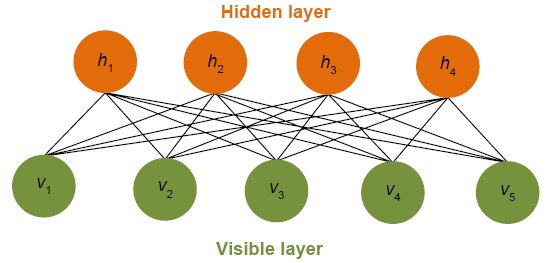
\includegraphics[scale=0.5]{images/RBM}
	\caption{ماشین بلتزمن محدود RBM}
	\label{fig1}
\end{figure}
RBM 
یک مدل بدون نظارت برای داده‌های باینری است که در دسته‌ی مدل‌های مولد احتمالاتی  قرار می‌گیرد. در این مدل با بیشینه کردن یک تابع انرژی، یا کمینه کردن مقدار منفی‌ آن که به صورت رابطه
\ref{eq1}
تعریف می‌‌شود، توزیع‌های احتمالی‌ موجود در داده‌های ورودی یاد گرفته می‌شود و از داده‌های ورودی ویژگی‌ استخراج می‌‌گردد. در رابطه‌ی
\ref{eq1}, $\theta = \{W, \textbf{a}, \textbf{b}\}$
مجموعه‌ی پارامترهای مدل است.
$W_{D*H}$
ماتریس وزن بین لایه‌ی ورودی و لایه‌ی پنهان است، که در آن
$D$
سایز بردار ورودی و
$H$
سایز لایه‌ی پنهان هستند.
$\textbf{a}$
بردار بایاس لایه‌ی ورودی با سایز
$D$
و
$\textbf{b}$
بردار بایاس لایه‌ی پنهان با سایز
$H$
است. در ساختار RBM توزیع‌های شرطی برای لایه‌های قابل مشاهده و پنهان به شکل روابط
\ref{eq2}
و
\ref{eq3}
هستند.
\begin{align}
\centering
\label{eq1}
E(\textbf{v},\textbf{h}) = -\sum_{i} \sum_{j} v_iW_{ij}h_j - \sum_i v_ia_i - \sum_j h_jb_j
\end{align}
\begin{align}
\centering
\label{eq2}
p(\textbf{h}|\textbf{v})=sigmoid(\textbf{v}W + \textbf{b})
\end{align}
\begin{align}
\centering
\label{eq3}
p(\textbf{v}|\textbf{h})=sigmoid(W\textbf{h} + \textbf{a})
\end{align}
در مدل RBM احتمال هر ترکیب
$(\textbf{v},\textbf{h})$
از رابطه‌ی
\ref{eq4}
بدست می‌‌آید که در آن
$Z(\theta)$
تابع قسمت‌بندی است که مقدار آن با استفاده از رابطه‌ی 
\ref{eq5}
محاسبه می‌شود و تضمین می‌کند که مقدار بدست آمده برای هر ترکیب
$(\textbf{v},\textbf{h})$
در رابطه‌ی 
\ref{eq4}
یک مقدار صحیح احتمالی‌ (بین ۰ و ۱) است. در این مدل احتمال هر بردار ورودی از رابطه‌ی
\ref{eq6}
بدست می‌‌آید.
\begin{align}
\centering
\label{eq4}
p(\textbf{v},\textbf{h}) = \dfrac{1}{Z(\theta)} e^{-E(\textbf{v},\textbf{h})}
\end{align}
\begin{align}
\centering
\label{eq5}
Z = \sum_{\textbf{v}, \textbf{h}}e^{-E(\textbf{v},\textbf{h})}
\end{align}
\begin{align}
\centering
\label{eq6}
p(\textbf{v}) = \sum_{h} \dfrac{1}{Z(\theta)} e^{-E(\textbf{v},\textbf{h})}
\end{align}
محدود بودن به حالت باینری برای داده‌های ورودی و همچنین طول ثابت برای آن‌ها دو محدودبت اساسی در مدل RBM استاندارد هستند. فرض کنید در مساله‌ای‌ که با آن سرو کار داریم هر داده‌ی ورودی دارای D ویژگی‌ است که هر یک از این ویژگی‌ها می‌‌توانند K مقدار داشته باشند. مدل RBM استاندارد توانایی کار کردن با یک چنین داده‌های ورودی را ندارد چرا که در آن داده‌های ورودی تنها می‌‌توانند یک بردار با طول ثابت و شامل ۰ و ۱ باشند. در این مدل جدید هر داده‌ی ورودی به صورت ماتریسی با سایز K*D در نظر گرفته می‌شود که همان‌طور که بیان شد D طول بردار ورودی یا همان تعداد ویژگی‌های مساله و K ماکسیمم مقداری است که هر ویژگی‌ می‌‌تواند داشته باشد. در این صورت تابع انرژی برای حالت
$\{\textbf{V},\textbf{h}\}$
به شکل رابطه‌ی
\ref{eq5}
تعریف می‌‌شود. همچنین رابطه‌ی
\ref{eq3}
به شکل رابظه‌ی
\ref{eq8}
تبدیل می‌شود.  دلیل استفاده از تابع
Softmax
در رابطه‌ی
\ref{eq8}
به جای تابع سیگموید که در مدل
RBM
استاندارد از آن استفاده می‌‌شود تغییر در ساختار ورودی و لایه‌ی قابل مشاهده است. با توجه به اینکه هر ویژگی‌ تنها یک مقدار از
$K$
مقدار ممکن را می‌‌تواند داشته باشد، لذا برای هر ستون در این ماتریس از تابع
Softmax
استفاده می‌گردد و یک توزیع اختمال چند جمله‌ای بدست می‌آید. سپس با تولید نمونه از این توزیع چند جمله‌ای مقدار آن ویژگی‌ تعیین می‌‌گردد.
\begin{align}
\centering
\label{eq7}
E(\textbf{V},\textbf{h})=-\sum_{i=1}^{D}\sum_{j=1}^{H}\sum_{k=1}^{K}W_{ijk}h_jv_{ik}-\sum_{i=1}^{D}\sum_{k=1}^{K}v_{ik}a_{ik} - \sum_{j=1}^{H}h_jb_j
\end{align}
\begin{align}
\centering
\label{eq8}
p(v_{ik}=1|\textbf{h})=\dfrac{exp(a_{ik}+\sum_{j=1}^{H}h_jW_{ijk})}{\sum_{k=1}^{K}exp(a_{ik}+\sum_{j=1}^{H}h_jW_{ijk})}
\end{align}
\begin{figure}[!t]
	\centering
	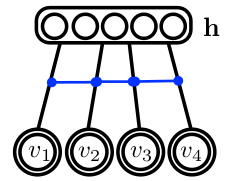
\includegraphics[scale=0.4]{images/RS}
	\caption{مدل Softmax Replicated}
	\label{fig2}
\end{figure}
برای مدل‌سازی موضوع پیش از آموزش مدل ابتدا یک لغت‌نامه از تمام کلمات متمایز در مجموعه اسناد ساخته می‌‌شود. حال در بردار ودرودی مقدار هر ویژگی‌ برابر با اندیس یکی‌ از کلمات دیکشنری است. به بیان دیگر هر سند ورودی پس از انجام پیش پردازش‌های لازم به یک دنباله از کلمات تبدیل می‌شود که هر کدام از این کلمات برابر با یکی‌ از کلمات دیکشنری هستند. به این ترتیب در ماتریس ورودی به مدل که یک ماتریس به انداز‌ه‌ی
$K*D$
است،
$K$
برابر با سایز دیکشنری و
$D$
نشان دهنده‌ی طول سند متنی است. در این حالت برای هر ستون مقدار سطر متناظر با اندیس آن کلمه در دیکشنری برابر با ۱ می‌‌شود و دیگر درایه‌های آن ستون همچنان صفر باقی‌ می‌‌مانند. در ابن مدل که 
Hinton
و
Salakhutdinov
آن را
RS
نامیدند و در شکل 
\ref{fig2}
نشان داده شده است، برای مدل کردن داده‌های متنی برای هر سند یک شبکه‌ی جدا می‌‌سازیم که به تعداد کلمات همان سند دارای واحد
Softmax
است. در این حالت ورودی دیگر یک ماتریس باینری نخواهد بود و به صورت برداری از تعداد کلمات موجود در آن سند است که می‌‌توانیم ترتیب را در آن‌ها نادیده بگیریم. رابطه‌ی محاسبه‌ی انرژی در این حالت به شکل رابطه‌ی
\ref{eq9}
است که در آن
$\hat{v}^k = \sum_{i=1}^{D}v_{ik}$
است. به عبارت دیگر
$\hat{\textbf{v}}$
برداری است با طول
$K$،
که 
$K$
همان سایز دیکشنری است و از محاسبه‌ی حاصل جمع سطر‌های ماتریس باینری ورودی بدست می‌‌آید. در این حالت روابط شرطی محاسبه‌ی لایه‌ی قابل مشاهده و لایه‌ی پنهان به شکل روابط
\ref{eq10}
و
\ref{eq11}
هستند. همانطور که مشاهده می‌‌شود در روابط
\ref{eq9}
و
\ref{eq11}
ترم بایاس برای لایه‌ی پنهان با سایز سند جاری نیز متناسب است. وجود این تناسب در پیاده‌سازی‌های تجربی‌ و هنگامی که اسناد با طول‌های متفاوت در مجموعه اسناد وجود دارد بسیار حیاتی است.
\begin{align}
\centering
\label{eq9}
E(\textbf{v},\textbf{h})=-\sum_{j=1}^{H}\sum_{k=1}^{K}W_{jk}h_j\hat{v}_{k}-\sum_{k=1}^{K}v_{k}a_{k} - D\sum_{j=1}^{H}h_jb_j
\end{align}
\begin{align}
\centering
\label{eq10}
p(v_{i}=w|\textbf{h})=\dfrac{exp(a_{w}+\sum_{j=1}^{H}h_jW_{wj})}{\sum_{k=1}^{K}exp(a_{w}+\sum_{j=1}^{H}W_{wj})}
\end{align}
\begin{align}
\centering
\label{eq11}
p(h_{j}=1|\textbf{v})=\sigma \left( Db_j + \sum_{k=1}^{K}W_{kj}\hat{v}_k \right)
\end{align}

مدل‌ها و حالت‌های معرفی شده تاکنون رویکردهایی هستند که پایه‌ی و اساس ساختار پیشنهادی در این مقاله هستند و با گسترش آن‌ها به شکلی که در ادامه بیان می‌شود مدل پیشنهادی در این مقاله بدست می‌آید. روبکرد معرفی‌ شده در این مفاله یک مدل مولد احتمالاتی نظارت شده 
بر پابه‌ی شبکه‌ی عصبی برای مدل‌سازی موضوع و احساس در داده‌های متنی است که در شکل
\ref{fig3}
نشان داده شده است. مشاهده می‌‌گردد که این روش نیز یک ساختار دو لایه دارد که در سمت لایه‌ی قابل مشاهده‌ی آن یک بردار متناظر با برچسب هر سند یا تعداد کلاس‌های موجود که در این پژوهش ما آن را به عنوان بردار متناظر با احساس هر سند تعبیر می‌کنیم به ساختار مدل اضافه شده است. بردار ورودی در این ساختار در قسمت قابل مشاهده یک بردار با طولی ثابت و به اندازه‌ی سایز دیکشنری یا همان تعداد کلمات متمایز در متن است که در آن تعداد تکرار کلمات مشخص شده است. در نظر گرفتن یک ماتریس ۲ بعدی برای هر سند ورودی به 
این معنی‌ است که جایگاه هر کلمه در متن دارای اهمیت است و ترتیب کلمات در هر سند درنظر گرفته می‌‌شود که این امر موجب بزرگ شدن فضای پارامتر‌های مساله (سه‌ بعدی شدن ماتریس وزن و دو بعدی شدن ماتریس بایاس برای لایه‌ی قابل مشاهده) و کند شدن فرآیند آموزش می‌‌گردد. علاوه بر این در بحث مدل‌سازی موضوع حضور و عدم حضور کلمات به همراه فرکانس تکرار آن‌ها دارای اهمیت است نه محل قرار گرفتن هر کلمه در متن، چرا که تمام مدل‌های بررسی‌ شده در این پژوهش و همچنین مدل پیشنهادی بر اساس کیسه کلمات رفتار می‌‌کنند که در آن ترتیب کلمات در نظر گرفته نمی‌‌شود.

در مدل پیشنهادی در این پژوهش و همچنین مدل
RS
هر سند به صورت یک بردار شامل تعداد کلمات به مدل وارد می‌‌شود. در این ساختار مانند آنچه که در شکل
\ref{fig3}
نشان داده شده است طول بردار ورودی برابر با سایز دیکشنری یا همان تعداد کلمات متمایز در مجموعه سند در نظر گرفته می‌‌شود که درایه‌های آن تعداد تکرار هر کلمه از دیکشنری در سند جاری را نشان می‌‌دهند. در این حالت در واقع وزن‌ها برای هر کلمه به اشتراک گذاشته می‌‌شوند، فارغ از اینکه این کلمه در کجای سند ورودی قرار دارد. به طور مثال برای کلمه‌ی‌
$n$ام 
دیکشنری یک وزن و یک بایاس تعریف می‌‌گردد و این کلمه در هر جای سند ورودی قرار داشته باشد وزنش تغییری نخواهد کرد و در فرآیند آموزش تنها یک وزن و یک بایاس برای هر کلمه یاد گرفته می‌‌شود. با توجه به ساختار مدل که در شکل
\ref{fig3}
نشان داده شده است، برای هر سند متنی یک بردار باینری که نشان دهنده احساس سند جاری است به عنوان ورودی به شبکه وارد می‌‌شود، و توزیع‌های موجود برروی کلمات مختلف در هر موضوع و همچنین احساس مرتبط با آن‌ها توسط مدل در لایه‌‌ی پنهان استخراج می‌‌شوند.

\begin{figure}[!t]
	\centering
	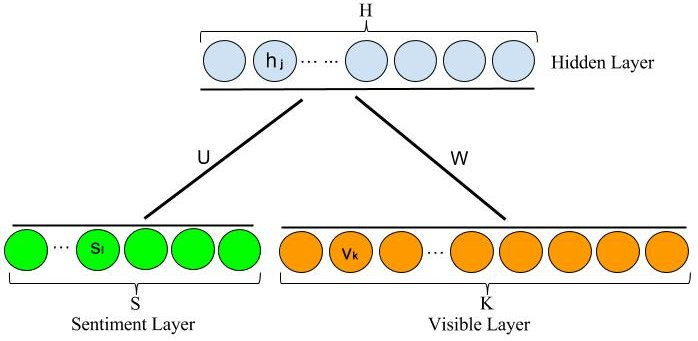
\includegraphics[scale=0.5]{images/SRS}
	\caption{مدل پیشنهادی مولد احتمالی احساس/موضوع}
	\label{fig3}
\end{figure}
	
برای محاسبه‌ی انرژی در مدل پیشنهادی ترم‌های مربوط به وزن و بایاس لایه‌ی احساس نیز در بدست آوردن مقدار نهایی مشارکت دارند. پس از محاسبه‌ی مقدار انرژی به کمک رابطه‌ی
\ref{eq12}،
با استفاده از فرمول
\ref{eq13}
	 احتمالی‌ که مدل به هر سند و ‌لایه‌ی احساس همراه با آن اختصاص می‌‌دهد، محاسبه می‌‌گردد. برای آموزش این مدل و بروزرسانی
پارامترهای شبکه که شامل ماتریس‌های وزن بین لایه‌ی قابل‌مشاهده و پنهان و همچنین لایه‌ی احساس و پنهان هستند و همچنین بایاس‌های هر سه‌ لایه از الگوریتم
CD
به شکل رابطه‌ی
\ref{eq14}
استفاده می‌‌شود. در رابطه
\ref{eq12}، $\theta=\{W, U, \textbf{a}, \textbf{b}, \textbf{c} \}$
مجموعه پارامتر‌های مدل است که در آن
$W_{K*H}$
ماتریس وزن بین بردار قابل مشاهده و لایه‌ی پنهان،
 $U_{S*H}$
ماتریس وزن بین لایه‌ی احساس و لایه‌ی پنهان و
$\textbf{a}$، $\textbf{b}$
و
$\textbf{c}$
به ترتیب بردار‌های بایاس لایه‌ی
قابل مشاهده، پنهان و احساس
هستند. لازم به ذکر است که
$K$
و
$H$
مانند آنچه که بیش از این ذکر کردیم به ترتیب سایز دیکشنری و طول لایه‌ی پنهان هستند و
$S$
به عنوان تعداد احساس موجود یا سایز بردار
احساس تعریف می‌‌شود.
\begin{align}
\label{eq12}
E(\textbf{V},\textbf{s},\textbf{h})=-\sum_{j=1}^{H}\sum_{k=1}^{K}W_{kj}h_j\hat{v}_{k}&-\sum_{j=1}^{H}\sum_{l=1}^{S}U_{lj}h_js_l\\\nonumber
&-\sum_{k=1}^{K}v_{k}a_{k} -\sum_{l=1}^{S}s_lc_l- D\sum_{j=1}^{H}h_jb_j
\end{align}
\begin{align}
\centering
\label{eq13}
p(\textbf{v},\textbf{s},\textbf{h}) = \dfrac{1}{Z} e^{-E(\textbf{v},\textbf{s},\textbf{h})} \Rightarrow
p(\textbf{v},\textbf{s}) = \dfrac{1}{Z} \sum_{h}  e^{-E(\textbf{v},\textbf{s},\textbf{h})} \ \ ,
Z = \sum_{\textbf{v}}\sum_{\textbf{s}}\sum_{\textbf{h}} e^{-E(\textbf{v},\textbf{s},\textbf{h})} 
\end{align}
\begin{align}
\centering
\label{eq14}
\triangle\theta = \alpha \left( E_{P_{data}}[\theta]-E_{P_{model}}[\theta]\right) \Rightarrow \theta_{t+1} = \theta_t + \triangle\theta
\end{align}

در مدل پیشنهادی مقادیر هر یک از لایه‌های قابل مشاهده، احساس و پنهان به کمک روابط
\ref{eq15}
تا
\ref{eq17}
محاسبه می‌شوند. در اینجا چون مقدار لایه‌ی پنهان به هر دو مقدار لایه‌ی قابل مشاهده و احساس وابسته است، لذا مشاهده می‌‌شود که در رابطه‌ی
\ref{eq17}
برای مقدار لایه‌ی پنهان از یک توزیع شرطی که وابسته به هر دو مقدار لایه‌های قابل مشاهده و احساس است نمونه گرفته می‌‌شود. اما با توجه به اینکه با داشتن مقدار لایه‌ی پنهان، بردارهای قابل مشاهده و احساس از یکدیگر مستقل شرطی هستند لذا در روابط
\ref{eq15}
و
\ref{eq16}
مقدار این دو بردار از یک توزیع شرطی که تنها به مقدار بردار
پنهان وابسته است نمونه گرفته می‌‌شوند.
\begin{align}
\centering
\label{eq15}
p(v_{i}=w|\textbf{h})=\dfrac{exp(a_{w}+\sum_{j=1}^{H}W_{wj}h_j)}{\sum_{k=1}^{K}exp(a_{w}+\sum_{j=1}^{H}W_{wj}h_j)}
\end{align}
\begin{align}
\centering
\label{eq16}
p(s_{l}=1|\textbf{h})=\dfrac{exp(c_{l}+\sum_{j=1}^{H}U_{lj}h_j)}{\sum_{l=1}^{S}exp(c_{l}+\sum_{j=1}^{H}U_{lj}h_j)}
\end{align}
\begin{align}
\centering
\label{eq17}
p(h_{j}=1|\textbf{v},\textbf{s})=\sigma \left( Db_j + \sum_{k=1}^{K}W_{kj}\hat{v}_k + \sum_{l=1}^{S}U_{lj}s_l \right)
\end{align}
با توجه به خصوصیات بیان شده برای تابع ,Softmax لذا همان‌طور که مشاهده می‌‌شود، در روابط
\ref{eq15}
و
\ref{eq16}
برای محاسبه‌ی مقادیر لایه‌های قابل مشاهده و احساس از یک تابع Softmax استفاده می‌‌گردد. در فرآیند آموزش با استفاده از الگوریتم CD
برای بدست آوردن مقدار بازسازی شده از لایه‌ی قابل مشاهده مشروط به بردار پنهان
از رابطه‌ی
\ref{eq15}
که به صورت Softmax است، استفاده می‌‌شود. در واقع دلیل اینکه این رابطه و رابطه‌ی
\ref{eq16}
برای لایه‌ی احساس به فرم تابع Softmax
هستند همین امر می‌‌باشد، که پس از محاسبه‌ی مقادیر این لایه‌ها مشروط به بردار پنهان نیاز به تولید نمونه و نمونه‌برداری از این مقادیر بدست آماده داریم. در نتیجه استفاده از تابع Softmax برای ما تضمین می‌‌کند که مقادیر محاسبه شده برای این دو بردار یک توزیع احتمالی‌ چندجمله‌ای خواهد بود که می‌‌توان به راحتی‌ از آن نمونه تولید کرد.

\section{آزمایش‌ها و ارزیابی مدل}
\section{نتیجه‌گیری}

%\newpage
%\bibliographystyle{plain-fa}
%\bibliography{reference.bib}
\end{document}